\section{User-Study}
\label{sec:userstudy}

To empirically evaluate the behavior of users of popular web applications and understand the patterns of their interactions, we conduct a user study. 
The main goal of this user study is to understand whether administrators use different subsets of the overall features available to them and would therefore benefit from differentially-debloated web applications.
Moreover, through this study, we analyze which features in the web applications in our dataset are commonly used among developers and administrators, and which features are relatively unpopular, used by only a fraction of administrators. 
% Figure~\ref{fig:environment_preparation} shows our high level approach for user data collection and debloating.

We hire the user-study participants by advertising paid projects on popular freelancing platforms, such as, Upwork and Fiverr~\cite{upwork, fiverr}. 
We interview freelancers with 2-10 years of expertise on web development and system administration. 
We specifically interviewed candidates who mentioned phpMyAdmin, WordPress, or Magento on their resume. 
We focused on these web applications since they were used in the ``Less is More'' study~\cite{lessismore}, allowing us to compare and contrast our findings with it. 

\subsection{User-Study Deliverables}
The task description for each project consists of an overview of the user-study, the background required to participate, and the expected deliverables. 
Moreover, we include the information about the consent to participate in our study and describe the information that we collect (i.e., server-side logs and code-coverage information). 

After interviewing the participants and reviewing their resumes, we hire 20 experts for each web application for a total of 60 experts on phpMyAdmin, WordPress, and Magento. 
We compensate the participants at the rate of \$15 per hour.
During the pilot experiments, we realized that not every freelancer is familiar with the concept of a user study. 
More importantly, to avoid future disputes, freelancers preferred to work on a predefined list of deliverables. 

Based on these observations, we define two milestones for our user study. 
First, we ask our participants to provide a list of web application features that they commonly use in their daily tasks and projects. 
Most of our participants listed both maintenance and administration tasks. 
Among the common tasks, we observed verification of the functionality of the website (e.g., registering as new customers, submitting orders, etc.), maintenance tasks (e.g., backups, importing data, etc.) and even search-engine optimization. 

For the second milestone, we ask our participants to spend one hour of their time on our instrumented web applications and perform the tasks that they listed earlier. 
This process provides them with the list of deliverables and expectations, and also enables us to validate their effort on this project. 

For freelancing platforms that provide a time-tracking utility, we use this feature to verify the participation of users together with cross-validating their task report with our code-coverage traces. 
For submissions that did not follow our guidelines (e.g., did not spend enough time, skipped the majority of tasks in the reports, etc.) we asked the participants to revise their submission. 

\textbf{IRB Approval} Since our experiments involved the assistance of real users, we obtained an Institutional Review Board (IRB) approval for our user study. 
Upon providing thorough details of our tasks and the human interactions, along with the information that we collect from the users, we obtained IRB approval on May 27, 2021. 

Throughout this user study, we interviewed over 110 individuals, some of whom decided not to participate in our study due to reasons such as non-recurring and short-term nature of our tasks, their busy schedule, etc.
Overall, we spent numerous weeks interviewing our participants and following up with them to ensure the timely delivery of their tasks. The cost of this experiment was approximately \$1,000, most of which was used to pay the administrators in our user study and the remainder to pay for domain names and the hosting of virtual machines on public clouds.

\subsection{Setup of Web Applications}

To facilitate the setup of web applications for our user-study participants, we prepared the following environments:

\begin{itemize}
    \item \textbf{phpMyAdmin} (version 5.1.0), with multiple pre-populated databases including the ones from WordPress and Magento web applications.
    \item \textbf{WordPress} (version 5.8) with an admin account, over 20 blog posts, multiple pages, and comments. 
    \item \textbf{Magento} (version 2.3.5) configured with an inventory of over 1,000 products. 
\end{itemize}

Each participant received their own instance with the admin credentials on a unique subdomain. 
We use a PHP code profiler to collect the usage traces from user interactions in the form of file and line-coverage data. 

\begin{figure}[t]
    \centering
    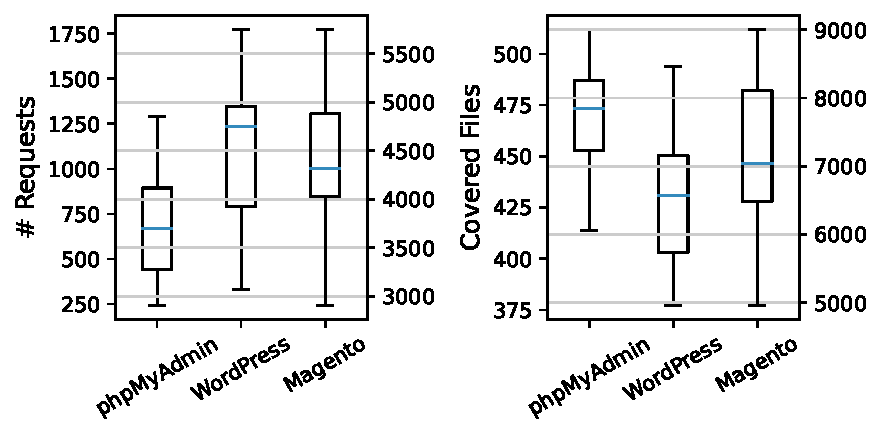
\includegraphics[width=0.8\linewidth]{figures/dbltr/userstudy_boxplots.pdf}
    \caption{Distribution of requests and covered files for user-study participants. For box plots of phpMyAdmin and WordPress refer the left y-axis and for Magento, refer to the right y-axis.}
	\label{fig:userstudystats}
\end{figure}

\subsection{Web Application Roles and Usage Patterns}

Looking at the usage traces (i.e., file and function coverage) of our user-study participants, we observe several patterns. 
Figure~\ref{fig:userstudystats} shows the distribution of PHP files invoked as the result of the requests of each user. 
We observe that for different web applications, administrators sent a range of requests. 
For instance, looking at phpMyAdmin, we observe that the majority of administrators sent between 500-800 requests with some outliers who sent as little as 240 and as many as 1,292 requests which invoked 388-512 distinct PHP files. 
This variance in the number of requests and the invoked files indicates the difference in the usage patterns of our participants. 

In this step, through the analysis of submitted reports and the code-coverage, we manually extracted common and unique access patterns. 
phpMyAdmin relies on its database backend (i.e., MySQL) to authentication users and enforce access-control. 
As a result, all users of phpMyAdmin have access to all features at the web application level (e.g., file upload, form submission, etc.), and access-control is only enforced when running SQL queries directly or indirectly through the UI. 
From our user-study logs, we observe a list of tasks that virtually all users performed. 
Creating new databases and tables, executing SQL queries, and using the import/export functionality of phpMyAdmin to backup and restore databases are among the commonly used features. 
On the contrary, only a subset of users changed the structure of existing tables and databases, or deleted data. 
From the export functionality, only a few users exported files with file extension other than SQL (e.g., CSV), and a few individuals used the provided filters to limit the query results. 

\begin{figure*}[t]
    \centering
    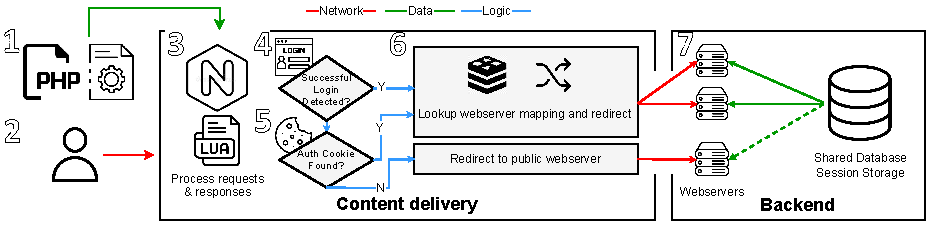
\includegraphics[width=\linewidth]{figures/dbltr/RoleModelsFlow.pdf}
    \caption{System Architecture of \dbltr{}. In Step 1, we provide the debloated web applications and user to cluster mappings to \dbltr{}'s content delivery module. User requests (2) are processed by \dbltr{}'s reverse-proxy (Step 3). After identifying the identity of the user (Steps 4-6), \dbltr{} internally routes the requests to the custom debloated web applications (Step 7).}
	\label{fig:system_architecture}
\end{figure*}

WordPress on the other hand ships with six hard-coded roles and the default role (i.e., Administrator) has the highest permission. 
WordPress administrators must rely on third-party plugins to customize the roles. 
By analyzing the usage traces of our WordPress user-study participants, we observe a group of users that focused on customizing themes and installing plugins. 
Another group focused on the website content, and their tasks included creation of new blog posts, along with adding tags and keywords to existing posts to enhance the SEO. 
Interestingly, only a few individuals used the import/export functionality of WordPress to backup blog post content, or setup the RSS/WXR feeds. 

Lastly, Magento provides the finest level of control over user permissions and roles. 
In this web application, administrators can define custom roles and assign permissions for individual sections of the administration panel. 
From our logs, we observe that the majority of users created new products, managed product inventory, and modified prices. 
Conversely, only a subset of users enabled sales promotions, gifts and shopping cart rules. 
Similarly, only \emph{some} users customized the front-end UI of the website.

Based on our observations, we determine that web applications must provide a baseline functionality to all of their users. 
Beyond this baseline, only a subset of the provided features are required by some and not all of their users (e.g., different export file formats), and certain features are left unused (e.g., phpMyAdmin GIS visualization). 
Previous work on debloating web applications only focused on the latter (i.e., debloating features that are not required by \emph{any} of the web application users). 
We identify the opportunity to provide customized debloating matching the needs of groups of users within a web application. 
Motivated by this observation, we discuss the design of our role-based debloating system in the next section. 
